\documentclass[twosided,a4,10pt]{article}
\usepackage[utf8]{inputenc}
\usepackage{amsmath}
\usepackage{amsfonts}
\usepackage{amssymb}
\usepackage{amstext}
\usepackage{mathrsfs}
\usepackage{textcomp}
\usepackage{german}
\usepackage{graphicx}
\usepackage[usenames,dvipsnames]{xcolor}
\usepackage{pifont}
\usepackage{nicefrac}
\usepackage{sectsty}
\usepackage{dblfnote}
\usepackage{verbatim}
% ------
% Fonts and typesetting settings
\usepackage[sc]{mathpazo}
\usepackage[T1]{fontenc}
\linespread{1.1} % Palatino needs more space between lines
\usepackage{microtype}
\subsectionfont{\fontsize{10}{15}\selectfont}

% ------
% Page layout
\usepackage[hmarginratio=1:1,top=32mm,columnsep=20pt]{geometry}
\usepackage[font=it]{caption}
\usepackage{paralist}
\usepackage{multicol}

%--------
%Footnote
\usepackage{footnote}
\usepackage{perpage} %the perpage package
\MakePerPage{footnote} %the perpage package command
\addtolength{\skip\footins}{2pc plus 5pt}
%------
%caption hack
\usepackage{caption}

%\DeclareCaptionType{faltung}[][List of equations]
%\captionsetup[faltung]{labelformat=empty}

% ------
% Abstract
\usepackage{abstract}
\renewcommand{\abstractnamefont}{\normalfont\bfseries}
\renewcommand{\abstracttextfont}{\normalfont\small\itshape}


% ------
% Titling (section/subsection)
\usepackage{titlesec}
%\renewcommand\thesection{\Roman{section}}
\titleformat{\section}[block]{\large\scshape\centering}{\thesection.}{1em}{}

% ------
% Clickable URLs (optional)
\usepackage[hyphens]{url}
\usepackage{hyperref}

% ------
% Header/footer
\usepackage{fancyhdr}
\pagestyle{fancy}
%	\fancyhead{}
%	\fancyfoot[C]{WIS WS 2017/18 $\cdot$
% Software Engineering $\cdot$ Prof. Dr. Dünnweber}
\fancyhead[R]{OTH Regensburg $\cdot$ Fakultät IM}
%	\fancyfoot[RO,LE]{\thepage}
\fancyfoot[L]{WIS $\cdot$ WS 2017/18}
\fancyfoot[R]{Prof. Dr. Dünnweber}
\fancyfoot[C]{\thepage}


% ------
% Maketitle metadata
\title{\vspace{-5mm}%
	\fontsize{20pt}{10pt}\selectfont
	\textbf{Inhaltsbasierte Musikempfehlung mit Convolutional Neuronalen Netzwerken}
}	
\vspace{-5mm}\date{}
\author{
	\large\begin{minipage}[t]{0.5\linewidth}
		\begin{center}
			\textsc{Weidhas Philipp}\\[2mm]
			\normalsize	Matr.nr: 123456\\
			\normalsize
			\href{mailto:philipp.weidhas@st.oth-regensburg.de}
			{philipp.weidhas@st.oth-regensburg.de}
		\end{center}
	\end{minipage}
	\begin{minipage}[t]{0.5\linewidth}
		\begin{center}
			\textsc{Wildgruber Markus}\\[2mm]
			\normalsize	Matr.nr: 123456\\
			\normalsize
			\href{mailto:markus.wildgruber@stud.oth-regensburg.de}
			{markus.wildgruber@stud.oth-regensburg.de}
		\end{center}
	\end{minipage}
}




%%%%%%%%%%%%%%%%%%%%%%%%
\begin{document}
	\maketitle
	\thispagestyle{fancy}
	\begin{multicols}{2}
		\begin{abstract}
			\noindent Hier kommt die Zusammenfassung...
		\end{abstract}
		\section{Einleitung}
		Im ersten Halbjahr des Jahres 2017 wurden 62\% der Einnahmen der amerikanischen Musikindustrie durch Streaming Plattformen\footnote[1]{wie Spotify, Apple Music, Pandora etc.} erzielt. Im Vergleich zum Vorjahr erhöhten sich dadurch die Einnahmen um 48\% auf 2.5\$ Milliarden \cite{friedlander}. Dieser Erfolg basiert nicht nur auf einer guten Verfügbarkeit der Lieder und einem günstigen Preis, sondern auch aufgrund automatischen Musikempfehlungsdiensten, welche dem Nutzer ein angenehmeres Konsumverhalten ermöglichen.\newline
		Obwohl Empfehlungsdienste in den letzten Jahren viel erforscht wurden, ist das Problem der Musikempfehlung sehr komplex. Neben einer großen Anzahl an verschiedenen Stilen und Genres, beeinflussen sowohl soziales und geographisches Umfeld, sowie der aktuelle Gemütszustand die Vorliebe eines Hörers. Diese Aspekte müssen, in einem Musikvorschlag, berücksichtigt werden. \cite{oord}\newline
		Neben der Empfehlung bestimmter Lieder sollen Empfehlungssysteme zusätzlich noch das Cold-Start Problem, sowohl bei einem Benutzer\footnote[2]{New User Problem (NUP)}, als auch bei einem Lied\footnote[3]{New Song Problem (NSP)} überwinden. Das Cold-Start Problem besteht darin, dass noch keine Bewertungen für ein Lied vorliegen, wodurch es auch nicht vorgeschlagen werden kann. Das selbe Problem gibt es bei einem neuen Benutzer: Diesem kann kein adäquater Vorschlag gemacht werden, da es an Information mangelt, welche Art von Musik ihm gefällt. \cite{celma}\\
		Mit Hilfe von Convolutional Neuronalen Netzwerken (CNN), können noch nicht alle Probleme überwunden werden. Sowohl das NSP als auch die Empfehlungsrate werden, durch die Verwendung eines CNN als Empfehlungssystem, verbessert.\newline\\
		Der weitere Verlauf der wissenschaftlichen Arbeit ist wie im Folgenden organisiert. Im 2. Abschnitt werden die Grundlagen der Musikempfehlung vorgestellt. Im 3. Kapitel wir der Aufbau von Neuronale Netze, soweit zwei Neuronale Netze für inhaltsbasierte Musikempfehlung beschrieben. Diese Arbeit, schließt im letzten Abschnitt, mit einem Vergleich der Ergebnisse der beiden Modelle.

		\section{Grundlagen der Musikempfehlung}
		In dem Gebiet der Musik Information Retrieval (MIR), gibt es vier Kategorien \cite{schedl}, die einen Einfluss, auf die Wahrnehmung, von ähnlicher Musik haben.\newline \textit{Musikmerkmale} sind Eigenschaften, welche aus dem Audiosignal eines Liedes extrahiert werden. Dazu zählen Aspekte wie der Rhythmus, die Melodie, die Harmonie oder die Stimmung eines Stückes.\newline
		Als \textit{Musikkontext} versteht man alle Aspekte, die nicht aus dem Audiosignal abgeleitet werden, sondern Informationen die über ein Musikstück bekannt sind. Beispielsweise Metadaten wie der Titel eines Lieds, das Genre, Name des Künstlers oder das Erscheinungsjahr.\newline
		Die \textit{Benutzereigenschaften} beziehen sich auf Persönlichkeitsmerkmale, wie Geschmack, musikalisches Wissen und Erfahrung oder den demographischen Hintergrund.\newline
		Im Unterschied dazu steht der \textit{Benutzerkontext}, der sich auf die aktuelle Situation des Hörers bezieht. Dabei wird er durch seine Umgebung, seiner Stimmung oder der aktuellen Aktivität beeinflusst. \cite{knees}\newline\\
		Es gibt verschiedene Methoden, die in Musikempfehlungssystemen verwendet werden: kollaboratives, merkmalsbasiertes, kontextbasiertes Filtern und die hybride Methode. Diese werden genutzt, um Informationen aus den genannten Eigenschaften zu gewinnen, um sie für Empfehlungen an den Nutzer zu verarbeiten. \cite{wang}
		\subsection{Matrix Factorization zu Musikbewertung}
		TODO glaube ich brauchen wir nicht, sollte bekannt sein TODO
		\subsection{Mel Frequency Cepstral Coefficients}
		Die Mel Frequency Cepstral Koeffizenten werden zur Analyse von Musikstücken verwendet und um Metadaten zuordnen zu können. Durch dieses Verfahren können die Tonhöhen, getrennt von der Sprache betrachtet werden. TODO genauer erklären? Todo
		\subsection{Bag of Words}
		BOW stellt ein klassisches Modell in der MIR da. Es stammt aus dem Feld der Textanalyse und wird dort Beispielsweise verwendet, um Dokumente automatisiert klassifizieren zu können. In diesem Modell wird ein Text als ansammlung von Wörtern gesehen. Diese Wörter werden gezählt und aufsummiert wie häufig das selbe Wort in einem Text auftritt. Über diese Häufung von Wörtern kann eine Klassifizierung dieses Textes erfolgen. TODO Zitat TODO In MIR wird dieses Modell in abgewandelter Form ebenfalls verwendet. Musikstücke werden mit Audiofeatures beschrieben. Abhängig davon wie häufig ein bestimmter Feature auf ein Lied zutrifft wird dies summiert.
		\subsection{Kollaborativer Filter}
		Kollaboratives Filtern prognostiziert Vorlieben eines Hörers, indem es aus unterschiedlichen Benutzer-Lied-Verhältnissen lernt. Es basiert auf der Annahme, dass Verhalten und Bewertungen andere Nutzer, auf eine vernünftige Vorhersage, für den aktiven Benutzer, schließen lassen \cite{celma}. Durch explizite\footnote[4]{ Bewertungen eines Nutzers} und implizite\footnote[5]{Beobachten des Konsumverhalten} Rückmeldung eines Hörers an das Empfehlungssystem, empfiehlt dieses neue Lieder, indem es Gemeinsamkeiten, auf Basis seiner Bewertungen, mit dem Nutzungsverhalten anderer Anwender, der gleichen Plattform, vergleicht \cite{mcfee}.\newline
		In der praktischen Umsetzung bedeutet dies: hört ein Anwender ein bestimmtes Musikstück. Dann werden ihm, von der Empfehlungsplattform, Lieder vorgeschlagen welche andere Nutzer, die ebenfalls dieses Lied hörten, hören. Dieses Verfahren geht davon aus, dass durch die Verbindung der Lieder durch vorhergehende Aufrufe eine gute Aussage darüber getroffen werden kann wie gut diese Stücke zusammen passen. Werden Lieder häufig nacheinander gehört, wird diese Verbindung höher bewertet und die Empfehlung häufiger ausgesprochen. Auch wird das Verhalten und der Musikgeschmack des Kunden selbst durch ein System analysiert, um so über Ähnlichkeiten der Kundenpräferenzen mit derer anderer, diesen wiederum bessere Empfehlungen aussprechen zu können. So werden Lieder einem Musikstil zugeordnet und so zielgerichtet dem Nutzer nahegelegt.\newline
		Verschiedene Studien (\cite{mcfee}\cite{barrington}) zeigen, dass KF alternative Methoden in der Genauigkeit übertrifft, weshalb es nicht nur im Bereich der Musikempfehlung als die erfolgreichste gilt.\newline
		\subsection{Merkmalbasierter Filter}
		%Als erstes wird nun ein genauerer Blick auf den inhaltsbezogenen Ansatz geworfen. Mittels diesem Verfahrens werden Nutze Musikstücke aufgrund aus Lieder gewonnener Informationen vorgeschlagen. Dies bedeutet im Detail dass aus den Musikstücken mittels verschiedenster Metriken die Audio Signale eines Liedes analysiert werden um Erkenntnisse über die Stimmung eines Musikstücks, die Frequenz oder Rhythmus zu erhalten. Auf Grund dieser Informationen können Stücke dem Konsumenten vorgeschlagen werden die einen gleichen oder sehr ähnlichen Inhalt bieten.
		\subsection{Kontextbasierter Filter}				
		\subsection{Hybride Methoden}
		Bei hybriden Methoden werden kollaborative, merkmalsbasierte und kontextbasierter Filter miteinander verknüpft. Dadurch kann ein besseres Empfehlungsergebnis mit weniger Nachteilen der einzelnen Methode erzielt werden. Meistens wird ein kollaborativer Filter mit einem der beiden anderen kombiniert.\newline
		Als \textit{gewichtet} wird eine hybride Methode bezeichnet, bei der Empfehlungsrate der einzelnen Methoden, durch eine Linearkombination zusammengerechnet wird. Das Ergebnis der Linearkombination stellt den Empfehlungswert eines Liedes dar. Durch unterschiedliche Gewichtung der Methoden, kann das Empfehlungsergebnis optimiert werden. Der \textit{wechselnde} Ansatz benutzt ein bestimmtes Kriterium anhand dessen es, die Methode zur Vorschlagbestimmung, wechselt. Dies kann beispielsweise dann der Fall sein, wenn der erste Filter kein zuverlässiges Ergebnis\footnote[6]{semantische Unterschiede} liefert. Dann wechselt das System den Filter und kann ein besseres Empfehlungsergebnis bekommen. Bei \textit{gemischten} hybriden Empfehlungen werden unterschiedliche Techniken\footnote[7]{meist kollaborativ mit inhaltsbasiertem Filter} miteinander vermischt. Dadurch kann für ein System mit inhaltsbasierten Filter, das Cold-Start Problem vermieden, werden.\newline
		Hybride Methoden können einige Nachteile von kollaborativen Filtern entfernen, allerdings stehen auch sie vor dem NUP. Dennoch sind hybride Methoden sehr beliebt, da Information über einen neuen Benutzer, schnell herausgefunden\footnote[8]{Datamining} werden oder durch Profilangaben, bereits nach der Registrierung, vorhanden sind. \cite{burke}
		\section{Neuronale Netze in der MIR}
		CNN sind durch das biologische Sehen inspiriert und konnten den ersten großen Erfolg, im Bereich der Bildklassifizierung \cite{alex}, verzeichnen. Trotzdem werden CNN auch in verschiedenen Audiobereich, wie der Spracherkennung \cite{graves}, sowie in der MIR mehr genutzt und erforscht.\newline
		Erste Forschungen im Bereich der MIR nutzen CNNs, um die Aufgabe der Musikgenre-Klassifizierung \cite{lee} zu untersuchen. Die Ergebnisse\footnote[9]{richtige Klassifizierung} zeigen, dass eine automatisierte Klassifizierung die herkömmliche Methode, MFCC, deutlich übertrifft. Das erste CNN für inhaltsbasierte Musikempfehlung \cite{oord}, benutzt zunächst eine Matrix-Faktorisierung, um Merkmalsvektoren\footnote[10]{Eigenschaften eines Musters in Vektordarstellung}, für alle Lieder, zu erhalten. Anschließend wird das Neuronale Netz für die Zuordnung, der Audio-Inhalte an die Merkmalsvektoren, genutzt. \cite{wang}\newline\\
		Im nachfolgenden Absatz werden die Schichten und das supervised\footnote[11]{Ausgabeergebnisse der Testdaten sind vorhanden} Training, eines CNN, beschrieben.
		\subsection{Convolutional Neuronalen Netze}
		In einer CNN Architektur werden drei Haupttypen von Schichten/Ebenen verwendet: Convolutional Layer (CL), Pooling Layer (PL) und Fully-Connected Layer (FCL). Jede Schicht besteht aus einer Anzahl von Knoten, die die Eingabedaten der Ebene wieder spiegeln. Knoten einer Schicht sind nur mit Knoten der nächsten Ebene verbunden. Diese Verbindung wird als Gewicht oder Parameter bezeichnet. Durch das Training von bekannten Daten und Ergebnissen werden diese Parameter automatisch angepasst. Anschließend ist das CNN fähig das Ergebnis unbekannter Daten zu errechnen.
		\subsubsection{Schichten eines Convolutional Neuronale Netzwerks}
		\begin{minipage}{0.45\textwidth}
			\centering
			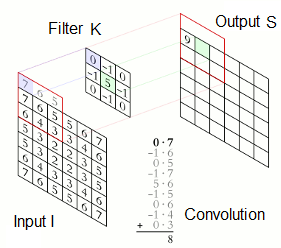
\includegraphics{img/faltung2.png}
			\captionof{figure}{Faltung einer 6x6 Matrix (mit Zero-padding) und einem 3x3 Filter \cite{wikipic}}
			\label{img:faltung}
		\end{minipage}\newline
		\subsubsection*{Convolutional Layer}
		In einem CL findet eine Faltung der Eingangsdaten, in Form einer Matrix und einem oder mehreren Filtern, statt. Ein Filter dient, beispielsweise zur Glättung oder zur Verkleinerung, der Daten. Eine Verkleinerung der Eingangsmatrix findet statt, wenn ein Filter ohne Zero-padding\footnote[12]{Eine Matrix wird, bei einer Faltung, am Rand, um Nullen erweitert.\\ Bsp. aus einer 7x7 Matrix wird eine 9x9 Matrix} verwendet wird. Die Parameter eines Filters werden zufällig initialisiert, können aber, mit Hilfe des Backpropagation Verfahrens (3.1.2) angepasst werden. Werden mehrere Filter auf die Eingangsdaten angewendet, ändert sich die Tiefe der gesamten Ausgangsmatrix entsprechend der Anzahl der Filter. \cite{karpathy}\newline
		In Abbildung \ref{img:faltung} ist die Eingabematrix \textit{I} eine 6x6 Matrix und \textit{K} ein 3x3 Filter. Die Ausgabematrix \textit{S} wir an den Stellen (i,j), durch die nachfolgende Gleichung, berechnet. Eine genauere Herleitung der Gleichung findet der Leser u. a. bei \cite{goodfellow}(328f).\newline\\	
		\begin{equation*}
		S(i,j) =(I \star K)(i,j)
		\end{equation*}
		\begin{equation*}
		(I \star K)(i,j) =\newline\sum_{m}^{}\sum_{n}^{}I(i+m,j+n)K(m,n)
		\end{equation*}\newline\\
		\subsubsection*{Pooling Layer}
		Ein PL wird zwischen zwei CL eingefügt. Ihre Funktion besteht darin, die Größe der Daten zu reduzieren und damit die Anzahl der Parameter für das nächste CL. Durch die Reduzierung wird die Berechnung des gesamten Netzwerkes beschleunigt. \cite{karpathy}\newline Ein PL wandelt die Ausgabe eines CL, durch eine statistische Zusammenfassung von nebeneinander liegenden Ausgängen, um. Verschiedene Methoden für ein Pl sind: Max Pooling \cite{zhou}, eine Übergabe der größten Zahl in einem rechteckigen Umfeld; die Durchschnittsberechnung des Umfeldes oder ein gewichteter Durchschnitt, basierend auf der Entfernung eines zentralen Punktes \cite{goodfellow}(355).\newline
		Abbildung \ref{img:pooling} zeigt einen 2x2 Max-Filter, der auf eine 4x4 Datenmatrix angewandt wird. Die Verschiebung oder Stride des Filters ist 2 dh. der Filter wird zunächst auf der y-Achse verschoben. Erreicht er dort das Ende, wird er um eine Stride auf der x-Achse verschoben und beginnt wieder mit der y-Verschiebung.\newline\\
		\begin{minipage}{0.4\textwidth}
			\centering
			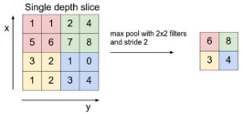
\includegraphics{img/pooling.png}
			\captionof{figure}{Maxpooling mit einem 2x2 Filter\cite{karpathy}}
			\label{img:pooling}
		\end{minipage}\newline
		\subsubsection*{Fully-Connected Layer}
		Ein oder mehrere geschachtelte FCL dienen als Ausgabeschicht. Jeder Knoten in einer FCL, hat eine Verbindung, zu allen Knoten, der vorherigen Schicht. Abhängig von der Problemstellung, Klassifizierung oder Regression, ist die Anzahl der Ausgabeknoten unterschiedlich. Bei einer Klassifizierung entspricht die Anzahl, in der letzten FCL, der der Klassen, die das CNN unterscheiden soll. Die Ausgabe der FCL ist ein Vektor in der jeder Eintrag, die Wahrscheinlichkeit, der jeweiligen Klasse, spiegelt. Bei einer Regression gibt das FCL einen Realwert aus. \cite{karpathy}
		\subsubsection{Training}
		CNNs werden, durch die Backpropagation Methode, trainiert. Backpropagation basiert auf dem Gradientenverfahren, welches versucht für die Fehlerfunktion \textit{E}, durch sukzessive Iteration der Parameter, ein globales Minimum zu finden, meistens aber nur ein lokales findet. Um das Minimum zu erreichen, werden die Werte der Gewichte \textit{w}\textsubscript{ij}, durch Verwendung der Kettenregel, der partiellen Ableitung, berechnet\footnote[13]{Ausgabeparameter \textit{o}, beliebige Anzahl an Knoten \textit{net} zwischen Ausgabe und \textit{w}}:
		\begin{equation*}
		\centering
		\frac{\partial\textit{E}}{\partial\textit{w}\textsubscript{ij}} = \frac{\partial\textit{E}}{\partial\textit{o}\textsubscript{j}} \frac{\partial\textit{o}\textsubscript{j}}{\partial\textit{net}\textsubscript{j}}  \frac{\partial\textit{net}\textsubscript{j}}{\partial\textit{w}\textsubscript{ij}} 
		\end{equation*}\newline
		Der neue Wert eines Parameters \textit{w}, zum Zeitpunkt \textit{t}, lässt sich durch folgende Formel berechnen:
		\begin{equation*}
		\centering
		\textit{w}(\textit{t}) = \textit{w}(\textit{t}-1) + \eta * \frac{\partial\textit{E}}{\partial\textit{w}} 
		\end{equation*}
		Die Lernrate $\eta$ ist eine Konstante, die definiert werden muss.\newline
		Anhand der Kostenfunktion, kann die Parameteranpassung und damit der funktionale Wert eines CNN, mit reellen Zahlen, dargestellt und verglichen werden. Diese Funktion \textit{C} lässt sich durch die Summe, über Trainingsbeispiele \textit{m} und einer Fehlerfunktion \textit{E}, hier die negativ conditional Log-Likelihood\footnote[14]{Abgeleitet von Maximum Likelihood, Dichtefunktion für Maximafindung}, darstellen: 
		\begin{equation*}
			\centering
			E(x,y) = -log p(y|x)
		\end{equation*}
		\begin{equation*}
			\centering
			\textit{C} = \frac{1}{m}\sum_{i=1}^{m}E(x\textsuperscript{i},y\textsuperscript{i})
		\end{equation*}
		Das Training eines Netzes ist abgeschlossen, wenn die Kostenfunktion minimal ist bzw. in einem gegebenen Zeitraum, keine bessere gefunden wird. \cite{goodfellow}(80ff,129ff)
		\subsection{Musikempfehlung mit Neuronalen Netzwerken}
			\subsection*{Anwendung eines CNN zur automatischen Musikempfehlung}
		
		Um das TODO Verzweigung TODO vorgestellt Problem der Semantischen Lücke zu lösen, kommt ein solches neuronales Netz zum Einsatz \cite{oord}. Dieser Ansatz wird wie folgt umgesetzt: das Netz wird darauf trainiert latente Faktoren aus einzelnen Musikstücken zu generieren, welche für eine Empfehlung verwendet werden. Dieses Verfahren wird anschließend im Vergleich mit einem konventionellen Ansatz, welcher dem Bag-of-Words Prinzip folgt. Daraus folgend wird beurteilt, inwiefern mittel CNN Eigenschaften zur spezifizierung des Nutzergeschmacks generiert und ausgewertet werden können.  In den folgenden Kapiteln wird auf diesen Ansatz nun genauer eingegangen.
		
		\subsubsection{Datenbasis}
		
		Als Datenbasis zur Umsetzung dieses neuen Ansatzes wurden verschiedene Musik Datensätze in Betracht gezogen. Diese stehen im zusammenhang mit dem Million Song Dataset TODO ABkürzung TODO, dieser Datensatz verfügt über Metainformationen und bereits analysierter Audio Informationen von einer Millionen Liedern. Ebenso ist dieser Datensatz öffentlich zugänglich und kann kostenlos heruntergeladen werden, des weiteren stellt dieser derzeit die größte Forschungsdatenbasis im Gebiet der Musikanalyse dar. Zwei Datensätze im Umfeld des MSD sind von besonderem Interesse, der Echo Nest Taste Profile Subset Datensatz und der The Last.fm Datensatz. Die Problematiken mit diesen Datensätzen, waren zum einen einem die schlechte Dokumentation der Generierung der Informationen und der Daten selbst, sowie das keine unverarbeiteten Musikquellen mitgeliefert werden. Das Problem der nicht vorhanden Rohdaten konnte beseitigt werden, in dem für 99\% des Datensatzes Musikschnipsel mit der Dauer von 29 Sekunden von 7digital.com bezogen wurden. Auf der Seite 7digital.com können einzelne Musikstücke 30 Sekunden lang Probegehört werden.TODO anders erläutern TODO TODO generell zu gleich mit dem Million Song Dataset Eintrag im Original Dokument, noch anpassen vll erweiter oder umändern TODO. Der ENTPS sticht durch seine Eigenschaft als größte, bereits mittels kollaborativen Filtern ausgwerteten, Informationsbasis hervor und bietet sich dadurch für ein Weiterverarbeitung mittels CNN an. Auch kann durch die größe der Daten eine realitätsnaher Versuch unternommen werden. Durch die Verwendung dieses Datensatzes, ist zu jedem Lied, pro Nutzer, die genaue Anzahl gespeichert, wie häufig das Stück vom Nutzer angehört wurde. 
		
		\subsubsection{Weighted matrix facorization}
		
		Wie bereits im Kapitel TODO VERWEIS TODO erklärt wird beim Kooperativen Filter angenommen das ein Nutzer ein Lied nur dann oft hört, wenn es im auch gefällt. Um diese Daten für ein Training des neuronalen Netztes zu verwenden, muss ein spezieller Algortihmus angewandt werden. Die üblichen Algorithmen, welche für ein Training eines neuronalen Netzes verwendet werden, dessen ziel eine Errechnung von Bewertungen haben, wie TODO BEISPIEL nennen TODO können nicht auf Basis dieser Daten zum Einsatz kommen, denn sie können nicht verarbeiten wenn für ein Lied keine Wertung vorliegt. tODO Satz auftrennen TODO Der Umstand das ein Lied keine Wertung erhalten hat, kann mehrere Gründe haben, unter anderem das ein Nutzer dieses Lied schlicht und ergreifen nicht kennt. Der Nutzer könnte allerdings das Lied bereits kennen, aus anderen Quellen, es nicht mögen und deshalb diesen Titel nicht anhören. Dies führt zu zwei unterschiedlichen Szenarien auf Grundlage der gleichen Wertung. Um diesen Umstand richtig bewerten zu können, muss der Algorithmus flexibel sein. Deshalb kommt ein weighted matrix factorization Algorithmus zum Einsatz, um die Informationen aus dem Taste Profile Subset zu verarbeiten. Diese Idee wurde angelehnt an den Versuch bei der Bewertung von Fernsehshows und deren automatisierter Empfehlung dem Nutzer gegenüber möglichst gute Ergebnisse zu erzielen. Es wurde gespeichert wie oft ein Nutzer ein Fernsehformat angesehen hat. Auch hier tritt der Fall auf das für Formate von einzelnen Nutzern keine Bewertungen vorlagen. Dies konnte mehrere Gründe haben: der Nutzer kennt das Format nicht, eine Sendung die er noch mehr schätzt kommt zur gleichen Sendezeit oder er mag die Sendung nicht. Folglich gibt es auch hier eine Ausgangswertung und drei Verschiedene Schlussfolgerungen sind möglich.
		
		Dieser, für implizite Bewertungen optimierter, WMF Algorithmus ist wie folgend aufgebaut:
		
		\begin{equation}\label{WMFAlgorithmus1}
		S(i,j) =(I \star K)(i,j)
		\end{equation}
		\begin{equation}\label{WMFAlgorithmus2}
		(I \star K)(i,j) =\newline\sum_{m}^{}\sum_{n}^{}I(i+m,j+n)K(m,n)
		\end{equation}\newline\\
		
		pui = I(Rui > 0),
		Cui = 1 + alphalog(1+Ehoch-1Rui)
		
		Rui steht für die Anzahl an Wiedergaben je Nutzer pro Lied. Für jedes dieser Nutzer-Song Paare, wird eine Präferenz Variable Pui und eine Confidence Variable Cui definiert. Cui bildet hierbei die Indikatorfunktion, Alpha und Epsylon bilden Hyperparameter. U soll für Nutzer (User) und I für das Musikstück (Item) stehen. Die Präferenz Variable beschreibt wie häufig ein Nutzer U einen Track I angehört hat. Entspricht der Wert 1, gefällt ihm dieses Lied. Die Confidence Variable wird genutzt um abbilden zu können wie aussagekräftig die Bewertung eines Liedes ist. Ein hoher Wert ergibt sich, wenn das Lied häufig gespielt wurde, ein niedriger Wert dagegen wenn ein Lied selten gespielt wird.
		
		Die Zielfunktion der WMF ist wie folgt gegeben:
		
		TODO ZEICHEN TODO ist der regularization Parameter, Xu ist der latente Faktor. U steht auch hier wieder für den Nutzer. Yi stellt den Latenten Vector für Musikstück i dar.Es baut auf einen confidence-gewichted quadtratische Fehler Term, sowie auf L2 als regulization Term mean squared error TODO umschreiben klingt kacke TODO Term auf.
		
		Beachten Sie, dass die erste Summe über alle Benutzer und alle Songs verteilt ist: im Gegensatz zur Matrix
		Faktorisierung für die Rating-Vorhersage, wobei die Begriffe den Benutzer-Element-Kombinationen entsprechen, für die
		Keine Bewertung verfügbar kann verworfen werden, wir müssen alle möglichen Kombinationen berücksichtigen. Wie
		Ein Ergebnis, bei dem ein stochastischer Gradientenabfall zur Optimierung verwendet wird, ist für einen Datensatz dieser Größe nicht praktikabel. Stattdessen wird eine effiziente Methode der alternierenden kleinsten Quadrate (ALS) verwendet, auch dies ist aus dem genannten Model angelehnt TODO CITE.
		
		
		%Note that the first sum ranges over all users and all songs: contrary to matrix
		%factorization for rating prediction, where terms corresponding to user-item combinations for which
		%no rating is available can be discarded, we have to take all possible combinations into account. As
		%a result, using stochastic gradient descent for optimization is not practical for a dataset of this size.
		%Hu et al. propose an efficient alternating least squares (ALS) optimization method, which we used
		%instead.
		
		\subsubsection{Extraktion und Analyse möglicher Faktoren aus dem Audiosignal}
		
		Um weitere Faktoren für eine Bessere Bewertung mit einfließen lassen zu können, müssen weitere Merkmale extrahiert und betrachtet werden. Die Vorhersage von Faktoren auf Grundlage von Audiosignalen eines Liedes lässt sich als Regressionsproblem definieren, die zu lernende Funktion muss eine Zeitreihe auf einen Vektor mit reellen Zahlen abbilden. Um dies zu lösen gibt es zwei Ansätze. Zum einen die Methode Bag-of-Words und das Training eines Convolutional Networks.
		
		
		
		Um das bereits vorgestellte BoW Modell verwenden zu können, müssen die Audiofeatures aus den Lieder extrahiert, in eine BoW Darstellung überführt und aggregiert werden. Dadurch können, mittels klassischer Regressionstechnik, die Merkmale auf Faktoren abgebildet werden. Um einen Vergleich mit dem Neuronalen Netz ziehen zu können wurde dieses Modell wie folgt umgesetzt:
		13 MFFCs wurden aus 1024 Audioschnipsel errechnet, des weiteren wurden unterschiede erster und zweiter Ordnung berechnet. Insgesamt wurden also 39 Koeffizienten errechnet. Mittels k-Means-Algorithmus zur Vektoreinquantisierung wurden 4000 Elemente gelernt und alle MFCC Vektoren dem nächsten Mittelwert zugeordnet. Anschließend wurde für jedes Lied gezählt, wie häufig ein Mittelwert ausgewählt wurde. Der daraus resultierende Vektor, repräsentierte als BoW-Feature ein einzelnes Lied. Abschließend wurde mittels Hauptkomponentenanalyse diese Features verkleinert. Aus diesen Features entstanden durch Lineare Regression und einem mehrlagigen Perzeptron, einem vereinfachten Neuronalem Netz, die Faktoren zur automatischen Musikempfehlung. %We also used it as input for the metric learning to rank (MLR)
		%algorithm [21], to learn a similarity metric for content-based recommendation. This was used as a
		%baseline for our music recommendation experiments, which are described in Section 5.2. TODO
		\newline
		
		
		Die zweite Möglichkeit ist es ein CNN zu trainieren. Faktoren welche durch den WMF, auf Basis der vorhanden Nutzerbewertungen, extrahiert werden, werden verwendet um die Vorhersagemodelle zu trainieren. Das WMF eignet sich hierfür besonders gut, da ein leistungsfähiges Optimierungsverfahren vorhanden ist. Um dieses Vorhaben umsetzen zu können, wurden 3 Erfolgsfaktoren definiert. Um das Netz gut trainieren zu können, ist es nötig auf eine große Menge an Trainingsdaten zurückgreifen zu können. Dies wird mittels der MSD, welche bereits vorgestellt wurde, abgesichert. Um das Problem das Vanishing Gradient Problem Todo erläutern und Verweisen TODO zu verrringern kommen rectified linear units zum Einsatz. Auch die Geschwindigkeit des Trainings an sich wird als kritisch betrachtet. Um ein schnelles Lernen zur ermöglichen, wurde der Lernvorgang parallelisiert und mittels GPU Unterstützung zur Berechnung optimiert. Eine GPU ist im Vergleich zu einer CPU in der Lage, in der gleichen Zeit, deutlich mehr Operationen durchzuführen, welche zum trainieren eines Neuronalen Netzes nötig sind. TODO GPU Unterstützung referenzieren TODO
		Das Trainining des CNN erfolgte in folgenden Schritten: Als erstes wurde wurden aus den Audiosignalen Zeit-Freuqzenz-Details extrahiert, um diese als Input für das Netz zu verwenden. Es handelten sich hierbei um Spektogramme, welche analog zum BoW-Modell aufgebaut waren. TODO satz überarbeiten TODO. Das Netz wurde mit 3 Sekundenlangen Audioschnipseln trainiert, welche zufällig aus den Songs entnommen wurden, dies sorgte für eine zusätzliche Beschleunigung der Trainingsgeschwindigkeit. Um die Features für den gesamten Song zu ermitteln wurden die Faktoren von aufeinanderfolgenden 3-Sekunden-Musikschnipseln gemittelt. 
		
		Da als Ergebniss der Zielfunktion die Faktoren als reelle Werte benötigt werden, muss der Quadratische Mittlere Fehler der vorhersagen reduziert werden.
		
		Latent factor vectors are real-valued, so the most straightforward objective is to minimize the
		mean squared error (MSE) of the predictions. Alternatively, we can also continue to minimize
		the weighted prediction error (WPE) from the WMF objective function. Let yi be the latent factor
		vector for song i, obtained with WMF, and y0i
		the corresponding prediction by the model. The
		objective functions are then ( represents the model parameters):
		
		%TODO hinzufügen ja nein TODO Convolutional neural networks are especially suited for predicting latent factors from music audio,
		%because they allow for intermediate features to be shared between different factors, and because their
		%hierarchical structure consisting of alternating feature extraction layers and pooling layers allows
		%them to operate on multiple timescales.
		
		\subsubsection{Versuchsaufbau und Durchführung vergleichender Tests}
		
		Nun werden die beiden Modelle, das BoW-Modell sowie das CNN-Modell, anhand deren Ergebnisse im Rahmen eines Experiments verglichen um die Leistungsfähigkeit des neuen Ansatzes bewerten zu können. Um die Qualität der Empfehlungen aber auch die extrahierten Faktoren an sich untersuchen zu können, wurden folgende drei Schritte unternommen.
		
		
		Untersuchung der Vielfältigkeit der latenten Faktoren zu untersuchen werden diese mit Tags für Lieder aus einem Tag-Prediktion-Verfahren TODO Verweis oder Erklärung TODO verglichen. Tags können Songs beschreiben, unter anderem Genre, Instrumentierung, Tempo, Stimmung und Erscheinungsjahr. Dieser Vergleich wurde auf basis aller 9,330 Lieder des Datensatzes erstellt  und die 50 Beliebtesten Tags aus der Last.fm Datenbank für jedes Stück extrahiert. Der vergleich ergab das die Vektoren einen erhöhte Empfehlungsgenauigkeit erbringen. tODO Verweis, stimmt das? TODo....
		
		%Wir haben WMF ausgeführt, um 50-dimensionale Vektoren für den latenten Faktor für alle 9.330 Lieder in der Untergruppe zu erhalten, und trainierte ein logistisches Regressionsmodell, um die 50 beliebtesten Tags aus dem Last.fm-Datensatz vorherzusagen für jedes Lied. Wir haben auch ein logistisches Regressionsmodell auf einer Bag-of-Word-Repräsentation der Audiosignale, die zunächst mit PCA verkleinert wurden (siehe Abschnitt 4.1). Wir verwendeten eine 10-fache Kreuzvalidierung und berechnete die durchschnittliche Fläche unter der ROC-Kurve (AUC) über alle Tags hinweg. Dies führte dazu in einer durchschnittlichen AUC von 0: 69365 für die audio-basierte Vorhersage und 0: 86703 für die Vorhersage basierend auf die latenten Faktorvektoren.
		
		
		Mittels quantitative Evaluation wird untersucht wie gut aus den Audioquellen der Lieder Faktoren extrahiert werden können. Um dies zu ermöglichen wurden die Faktoren verwendet um damit die ein Empfehlungssystem umzusetzen. Für jeden Nutzer u und jeden Song i der Datenbasis wurde eine Wertung xTuYi errechnet und das Lied mit dem höchten Wert als erstes vorgeschlagen. Zum Vergleich wurden ebenfalls für Nutzer und Songs mittels Bag-of-Words System Wertungen gefunden. In diesem Modell wurden alle Wertungen für einen gegebenen Nutzer in eine Durchnschnitts-Ähnlichkeits-Wertung umgerechnet basierend auf alle Lieder welche dieser Nutzer bereits hörte.
		
		%Um quantitativ zu beurteilen, wie gut wir latente Faktoren aus Musik-Audio vorhersagen können, haben wir die Vorhersagen verwendet von unseren Modellen für Musikempfehlung. Für jeden Benutzer und für jeden Song in der Test-Set, berechneten wir den Score xT U yi, und empfahl die Songs mit den höchsten Punktzahlen zuerst. Wie bereits erwähnt, lernten wir auch eine Liedähnlichkeitsmetrik auf der Bag-of-Word-Darstellung mit metrisches Lernen zum Rang. In diesem Fall werden die Bewertungen für einen bestimmten Benutzer durch Durchschnittsbildung berechnet Noten über alle Songs, die der Benutzer gehört hat.
		
		
		Um die Faktorvektoren vorhersagen zu können, wurde jeweils wie folgt verfahren:
		Eine Lineare Regressiont welche auf den Bag-Of-Words ansatz trainiert wurde. Ein MLP trainiert auf ebenfalls dem gleichen BoW-Modell. Ein CNN, welches auf log-skalierten Mel-Spektogrammen trainiert wurde, um den den Mittleren quadratischen Fehler der Vorhersagen zu reduzieren. Abschließend wurde das gleiche CNN trainiert um den WPE aus dem WMF zu verringern.
		
		%Die folgenden Modelle wurden verwendet, um latente Faktorvektoren vorherzusagen: Lineare Regression, trainiert auf der in Abschnitt 4.1 beschriebenen Bag-of-words-Repräsentation. Ein mehrschichtiges Perzeptron (MLP) trainiert auf der gleichen Wort-zu-Bild-Darstellung. Ein konvolutionelles neuronales Netzwerk, das auf log-skalierten Mel-Spektrogrammen trainiert wurde, um den Mittelwert zu minimieren quadrierter Fehler (MSE) der Vorhersagen. Das gleiche faltungsneurale Netzwerk, trainiert um den gewichteten Vorhersagefehler zu minimieren (WPE) aus dem WMF-Ziel stattdessen.
		
		Für unsere ersten Experimente verwendeten wir eine Untergruppe der Datensatz, der nur die 9.330 beliebtesten Lieder enthält und Abhören von Daten für nur 20.000 Benutzer. Wir haben 1.881 benutzt Lieder zum Testen. Für die anderen Experimente haben wir verwendet alle verfügbaren Daten: Wir haben alle Lieder verwendet, die wir verwenden Daten für und dass wir einen Audioclip herunterladen konnten für (382,410 Lieder und 1 Million Benutzer insgesamt, 46.728 Lieder wurden zum Testen verwendet).
		
		Wir geben die durchschnittliche Durchschnittsgenauigkeit an (mAP, abgeschnitten bei 500 Empfehlungen pro Benutzer) und der Bereich unter der ROC-Kurve (AUC) der Vorhersagen. Wir haben alles bewertet Modelle auf der Teilmenge, unter Verwendung von latenten Faktorvektoren mit 50 Dimensionen. Wir haben das Faltungsneuronal verglichen Netzwerk mit linearer Regression auf der Bag-of-Word-Darstellung auf dem gesamten Datensatz, unter Verwendung von Vektoren mit latenten Faktoren mit 400 Dimensionen. Ergebnisse sind in den Tabellen 2 bzw. 3 gezeigt.
		
		
		Bei der Untergruppe scheint die Vorhersage der latenten Faktoren den metrischen Lernansatz zu übertreffen. Verwenden Ein MLP anstelle einer linearen Regression führt zu einer geringfügigen Verbesserung, aber die Einschränkung ist hier eindeutig die Textdarstellung der Wörter. Die Verwendung eines konvolutionellen neuronalen Netzwerks führt zu einem anderen große Leistungssteigerung. Wahrscheinlich liegt das daran, dass die Bag-of-Word-Darstellung nicht funktioniert reflektieren jede Art von temporaler Struktur.
		
		Interessanterweise führt das WPE-Ziel nicht zu einer verbesserten Leistung. Vermutlich ist das so Die Gewichtung bewirkt, dass die Bedeutung der Lieder ihrer Popularität proportional ist. Im Mit anderen Worten, das Modell wird ermutigt, latente Faktorvektoren für populäre Lieder aus zu prognostizieren das Training lief sehr gut, auf Kosten aller anderen Songs.
		
		Auf dem vollständigen Datensatz, der Unterschied zwischen den Beutelwörtern Ansatz und das konvolutionelle neuronale Netzwerk ist viel ausgeprägter. Beachten Sie, dass wir nicht trainiert haben MLP auf diesem Datensatz aufgrund der geringen Differenz in der Leistung mit linearer Regression auf der Teilmenge. Wir auch eingeschlossene Ergebnisse, wenn die latenten Faktorvektoren erhalten werden aus Nutzungsdaten. Dies ist eine obere Grenze für was ist erreichbar, wenn man sie aus dem Inhalt vorhersagt. Dort ist eine große Lücke zwischen unserem besten Ergebnis und diesem theoretischen Maximum, aber das ist zu erwarten: wie bereits erwähnt, viele Aspekte der Songs, die die Präferenz der Nutzer beeinflussen kann unmöglich nur aus Audiosignalen extrahiert werden. Insbesondere können wir die Popularität von die Lieder, die AUC und mAP erheblich beeinflussen Punkte.
		
		
		
		Eine Bewertung der Qualität der gefundenen Faktoren, kann nicht nur auf der Betrachtung der Genauigkeit des Empfehlungssystems bezogen werden sondern sollten auch die vorgeschlagenen Lieder als Ergebniss betrachtet werden. Ein Vergleich der mittels CNN vorhergesagten Faktoren empfohlenen Liedern einerseits und die TODO welche Sinds Todo anderseits ergaben folgendes: Liedermengen sind sehr unterschiedlich, nur wenige Teilmengen vorhanden. Allerdings sind beide Ergebnissmengen ein gutes Ergebniss und die mittel CNN-Modell gefundenen Liedermenge ist etwas abwechslungsreicher was für ein Empfehlungssystem als Vorteil zu sehen ist.
		
		%Die Bewertung von Empfehlungssystemen ist eine komplexe Angelegenheit und Genauigkeitsmetriken selbst liefern nicht genügend Einblick ob die Empfehlungen gut sind. Um dies festzustellen, haben wir auch einige durchgeführt qualitative Experimente an der Teilmenge. Für jedes Lied suchten wir nach ähnlichen Songs durch Messen die Kosinusähnlichkeit zwischen den vorhergesagten Nutzungsmustern. Wir haben die prognostizierten Nutzungsmuster verglichen Verwendung der mit WMF erhaltenen (50 Dimensionen), bei denen latente Faktoren verwendet werden mit einem konvolutionellen neuronalen Netzwerk vorhergesagt. Ein paar Lieder und ihre besten Übereinstimmungen zu beiden Modellen sind in Tabelle 4 gezeigt. Wenn die vorhergesagten latenten Faktoren verwendet werden, sind die Übereinstimmungen meist unterschiedlich, aber die Ergebnisse sind in dem Sinne durchaus sinnvoll, dass die passenden Songs wahrscheinlich sind um das gleiche Publikum anzusprechen. Außerdem scheinen sie ein bisschen abwechslungsreicher zu sein, was nützlich istEigenschaft für Empfehlungssysteme.
		
		%Nach McFee et al. [5] visualisierten wir auch die Verteilung der prognostizierten Nutzungsmuster in zwei Abmessungen mit t-SNE [27]. Einige Nahaufnahmen sind in Abbildung 1 dargestellt. Cluster von Songs, die ansprechen zu demselben Publikum scheinen sich recht gut erhalten zu haben, obwohl die latenten Faktorvektoren für alle Lieder wurden von Audio vorhergesagt.
		
		
		\subsection{Hybride Musikempfehlung mit einem Neuronalen Netzwerk}
		Im Unterschied, zu der davor dargestellten Forschung (3.2), wird nun ein Deep Belief Netzwerk(DBN) verwendet, um ein hybrides inhaltsbasiertes Musikempfehlungssystem zu entwickeln. Im Gegensatz zu einem CNN, nutzt ein DBN ein so genanntes Pretraining\footnote[15]{Parameter von Model A wird für das neue Model B verwendet} als Parameterinitialisierung. Bisherige inhaltsbasiertes Systeme verfolgen typischerweise einem zweistufigen Ansatz: Zunächst extrahieren sie aus Audioinhalte den MFCC Koeffizienten; anschließend prognostizieren sie Musikpräferenzen, eines Nutzers. Das nachfolgende Modell führt diese beiden Schritte simultan und automatisch aus. \cite{wang}\newline
		Das hybride Modell basiert auf einem hierarchisch linearen Modell mit einem Deep Belief Netzwerk (HLDBN), das zunächst erläutert wird, um anschließend die Funktionsweise, des hybriden System,s darzustellen.
		\begin{minipage}{0.45\textwidth}
			\centering
			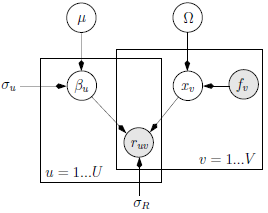
\includegraphics{img/hlmdbn.png}
			\captionof{figure}{Hierarchisches lineares Modell eins Deep Belief Netzwerks \cite{wang}}
			\label{img:hlmdbn}
		\end{minipage}
		\subsubsection{Hierarchisches lineares Modell mit einem Deep Belief Netzwerk}
		Das in Abbildung \ref{img:hlmdbn} gezeigte Modell ist wie folgt definiert: \textit{f\textsubscript{v}} sind Musikmerkmale eines Liedes \textit{v}, die durch den Merkmalsvektor x\textsubscript{v} automatisch errechnet werden. Die bevorzugte Musik eines Benutzers \textit{u} wird as Vektor $\beta$\textsubscript{u} bezeichnet. $\Omega$ bezeichnet die Parameter, die das DBN lernt. Die Bewertung \textit{r\textsubscript{xv}}, die ein Nutzer einem Lied \textit{v} gibt, ist ein Skalarprodukt von \textit{x\textsubscript{v}} und $\beta$\textsubscript{u}. Durch $\sigma$\textsubscript{R} wird die Varianz aller Bewertungen des Nutzers betrachtet. $\mu$ repräsentiert den allgemeinen Musikgeschmack aller Benutzer, wobei $\sigma$\textsubscript{u} die Varianz des einzelnen Nutzers definiert. Alle Benutzer und Lieder Paare werden als \textit{I} bezeichnet. Für eine Regularisierung der Werte wird die Gaußsche Normalverteilung $\mathcal{N}$ verwenden.\footnote[16]{$\mathcal{N}$(a,b) ist die Normalverteilung mit Mittelwert a und Varianz b. x $\sim$ p zeigt, dass x die Verteilung p erfüllt}\newline
		Das Modell ist wie folgt formuliert:\newline
		\begin{equation*}
			\centering
			\textit{r\textsubscript{xv}}\sim\mathcal{N}(\beta'\textit{x\textsubscript{v}},\sigma\textsuperscript{2}\textsubscript{R})
		\end{equation*}
		\begin{equation*}
		\centering
			\beta\sim\mathcal{N}(\mu,\sigma\textsuperscript{2}\textsubscript{u}\textit{I})
		\end{equation*}
		\begin{equation*}
			\textit{x\textsubscript{v}} = DBN(\textit{f\textsubscript{v}};\Omega)
		\end{equation*}\newline\\
		Für das Training des Systems wird im Unterschied zu einem CNN zunächst ein unsupervised\footnote[17]{Ausgabeergebnisse der Testdaten sind nicht vorhanden} Training durchgeführt um die Knoten zu initialisieren. Anschließend findet ein supervised Training zur Optimierung der Parameter statt. Als Optimierungsmethode wird das stochastische Mini-Batch\footnote[18]{nur ein kleiner Teil der vorhandenen Daten wird trainiert} Verfahren mit Backpropagation genutzt, um ein Overfitting\footnote[19]{Spezialisierung} des Modells zu vermeiden. Nach der Lernphase kann die Bewertung \textit{r\textsubscript{xv}} eines Benutzers \textit{u} über ein Lied \textit{v} geschätzt werden, wodurch diesem neue Lieder empfohlen werden können. \cite{wang}
		\subsubsection{Hybrides Modell mit einem Deep Belief Netzwerk}
		Basiert auf dem HLDBM wird das in Abbildung \ref{img:hybrid} gezeigte Modell um einen kollaborative Filter erweitert, um eine noch bessere Empfehlungsrate zu erhalten.
		\begin{minipage}{0.45\textwidth}
			\centering
			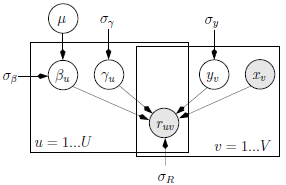
\includegraphics{img/hybrid.png}
			\captionof{figure}{Hybrides Empfehlungs Modell \cite{wang}}
			\label{img:hybrid}
		\end{minipage}\newline\\
		Die Musikmerkmale eines Liedes \textit{x}\textsubscript{v} wird wie in (3.4.1) berechnet. Die bevorzugte Musik eines Nutzers wird als $\beta$\textsubscript{u} bezeichnet. Der kollaborative Teil: $\gamma$\textsubscript{u} stellt einen Vektor über alle Benutzer \textit{u} dar; \textit{y}\textsubscript{v} den Vektor über alle Lieder \textit{v}. $\beta$\textsubscript{u}, $\gamma$\textsubscript{u} und \textit{y}\textsubscript{v} werden gemeinsam, durch das Neuronale Netzwerk, anhand der Trainingsdaten gelernt. Die Empfehlungsrate \textit{r}\textsubscript{uv} ergibt sich aus der Summe der Skalarmultiplikationen  $\gamma$'\textsubscript{u}\textit{y}\textsubscript{v} und  $\beta$'\textsubscript{u}\textit{x}\textsubscript{v}. Die A-priori-Wahrscheinlichkeit\footnote[20]{Anfangswahrscheinlichkeit} werden durch die folgenden Formeln definiert:\newline
		\begin{equation*}
		\centering
		\textit{r\textsubscript{xv}}|\beta\textsubscript{u},\textit{x}\textsubscript{v},\gamma\textsubscript{u},\textit{y}\textsubscript{v},\sigma\textsubscript{R}\sim\mathcal{N}(\beta'\textsubscript{u}\textit{x}\textsubscript{v} + \gamma'\textsubscript{u}\textit{y}\textsubscript{v},\sigma\textsubscript{R}\textsuperscript{2})
		\end{equation*}
		\begin{equation*}
		\centering
		\beta\textsubscript{u}|\sigma\textsubscript{$\beta$}\sim\mathcal{N}(\mu,|\sigma\textsubscript{$\beta$}\textsuperscript{2}I)
		\end{equation*}
		\begin{equation*}
		\centering
		\gamma\textsubscript{u}|\sigma\textsubscript{u}\sim\mathcal{N}(0,|\sigma\textsubscript{$\gamma$}\textsuperscript{2})
		\end{equation*}
		\begin{equation*}
		\centering
		\textit{y}\textsubscript{v}|\sigma\textsubscript{v}\sim\mathcal{N}(0,|\sigma\textsubscript{y}\textsuperscript{2})
		\end{equation*}\newline
		Die Fehler Funktion des Modells wird auch mit Hilfe der Backpropagation minimiert. Um Zeit zu sparen, können die Werte für $\gamma$\textsubscript{u} und \textit{y}\textsubscript{v} durch eine PMF berechnet und als Initialwerte verwendet werden. \cite{wang}\newline
		Um Informationen aus einem Lied, als Eingabeparameter für das DBN, nutzen zu können, muss dieses in einen Vektor umgewandelt werden. Dies geschieht in verschiedenen Schritten. In \cite{wang} werden alle Lieder in ein .wav Dateiformat, mit einer 8 kHz Abtastrate und 16 Bit Tiefe, umgewandelt. Aus den einzelnen Liedern wird ein 5 Sekunden Abschnitt genutzt, der in ein 166x120 Spektrogramm umgewandelt wird. Anschließend wird eine Hauptkomponentenanalyse\footnote[21]{Zusammenhang der Darstellung einer Menge an Variablen durch wenige Faktoren} durchgeführt, wodurch sich ein Vektor für den Liedabschnitt ergibt.
		\section{Vergleich der vorgestellten Modelle}
		Abschließend wird nun ein Vergleich zwischen dem vorgestellten CNN Ansatz einerseits und dem danach folgendem DBN gezogen. In Versuchen \cite{oord} wurde festgestellt das dass CNN Model einem BOW System überlegen ist und eine bessere Empfehlungsrate erreicht. Das anschließend erläuterte  Versuchsmodel, welches mittels DBN einen hybriden Methode verfolgt, konnte im direkten Vergleich zu CNN eine nochmals verbesserte Empfehlungsgenauigkeit erreichen. Vergleichende Versuchsreihen \cite{wang} haben folgendes festgestellt: ein nicht hybrider Ansatz welcher allein auf Training der beiden Netze ergab, dass das vorgestellte HLDBN Modell genauere Ergebnisse lieferte als das vorgestellte CNN. Die Integration der beiden Modelle in einen hybriden Aufbau ergab wiederum ebenso dass der Einsatz des HLDBN Netzes zu genaueren Empfehlungsraten führte als die Verknüpfung von CNN und CF. Die Empfehlungsraten für bereits bekannte Lieder, konnten somit im Vergleich zu klassischen Ansätzen verbessert werden. Auch das bereits eingeführte Problem des NSP konnte durch den Einsatz Neuronaler Netze gelöst werden.  Sowohl der Einsatz des CNN als auch der des HLDBN Netzes führen hierbei zum Erfolg.
		Sowohl der im Punkt 3.2 vorgestellte Ansatz mittels eines CNNs sowie der in Punkt 3.3 erläuterte Ansatz mit Einsatz eines hybriden DBN Netzwerkes eine gute Möglichkeit zur automatisierten Musikempfehlung. Beide Verfahren haben in Rahmen von Versuchen bewiesen, dass sie sowohl zuverlässig sind, aber auch das sie einen klassisches Verfahren wie ein BoW-System 
		%\bibliographystyle{abbrvdin}
		\bibliographystyle{unsrt}
		\bibliography{lit}
	\end{multicols}
\end{document}
